---
title: ''
fontfamily: mathpazo
fontsize: 10pt
geometry: margin=1mm
linestretch: 0.1
classoption:

pagenumbering: FALSE
whitespace: none
output:
  pdf_document:
    toc: FALSE
    number_sections: FALSE

header-includes:
\usepackage{multicol}
\usepackage{calc}
\usepackage{ifthen}
\usepackage[landscape]{geometry}
\usepackage{amsmath,amsthm,amsfonts,amssymb}
\usepackage{color,graphicx,overpic}
\usepackage{hyperref}
\usepackage{graphicx}
---
%\documentclass[10pt,landscape]{scrartcl}

% This sets page margins to .5 inch if using letter paper, and to 1cm
% if using A4 paper. (This probably isn't strictly necessary.)
% If using another size paper, use default 1cm margins.
\ifthenelse{\lengthtest { \paperwidth = 11in}}
    { \geometry{top=.5in,left=.5in,right=.5in,bottom=.5in} }
    {\ifthenelse{ \lengthtest{ \paperwidth = 297mm}}
        {\geometry{top=1cm,left=1cm,right=1cm,bottom=1cm} }
        {\geometry{top=1cm,left=1cm,right=1cm,bottom=1cm} }
    }

% Turn off header and footer
\pagestyle{empty}

% Redefine section commands to use less space
\makeatletter
\renewcommand{\section}{\@startsection{section}{1}{0mm}%
                                {-1ex plus -.5ex minus -.2ex}%
                                {0.5ex plus .2ex}%x
                                {\normalfont\large\bfseries}}
\renewcommand{\subsection}{\@startsection{subsection}{2}{0mm}%
                                {-1explus -.5ex minus -.2ex}%
                                {0.5ex plus .2ex}%
                                {\normalfont\normalsize\bfseries}}
\renewcommand{\subsubsection}{\@startsection{subsubsection}{3}{0mm}%
                                {-1ex plus -.5ex minus -.2ex}%
                                {1ex plus .2ex}%
                                {\normalfont\small\bfseries}}
\makeatother

% Define BibTeX command
\def\BibTeX{{\rm B\kern-.05em{\sc i\kern-.025em b}\kern-.08em
    T\kern-.1667em\lower.7ex\hbox{E}\kern-.125emX}}

% Don't print section numbers
\setcounter{secnumdepth}{0}


\setlength{\parindent}{0pt}
\setlength{\parskip}{0pt plus 0.5ex}

%My Environments
\newtheorem{example}[section]{Example}
% -----------------------------------------------------------------------


\newcommand{\sect}[1]{\vspace{1mm}\textbf{#1}\\}


\author{Gerold, Edited by Shengliang}
\begin{document}
\raggedright
\footnotesize
\begin{multicols}{3}


% multicol parameters
% These lengths are set only within the two main columns
%\setlength{\columnseprule}{0.25pt}
\setlength{\premulticols}{1pt}
\setlength{\postmulticols}{1pt}
\setlength{\multicolsep}{1pt}
\setlength{\columnsep}{2pt}

\begin{center}
     \Large{\underline{Linear Algebra Cheat Sheet}} \\
\end{center}


\section{Matrices}
\subsection{basic operations}
transpose: $[A^\mathrm{T}]_{ij} = [A]_{ji}$: ``mirror over main diagonal"\\
conjungate transpose / adjugate: 
$A^* = (\overline{A})^\mathrm{T} = \overline{A^\mathrm{T}}$\\
``transpose and complex conjugate all entries"\\(same as transpose for real matrices)\\

multiply: $A_{N \times K} * B_{K \times M} = M_{N \times M}$\\
invert: $\begin{bmatrix}
a & b \\ c & d \\ 
\end{bmatrix}^{-1} =
\frac{1}{\det(\mathbf{A})} \begin{bmatrix}
\,\,\,d & \!\!-b \\ -c & \,a \\ 
\end{bmatrix} =
\frac{1}{ad - bc} \begin{bmatrix}
\,\,\,d & \!\!-b \\ -c & \,a \\ 
\end{bmatrix}$\\



\subsection{determinants}
$\det(A) = \sum_{\sigma \in S_n} \text{sgn}(\sigma) \prod_{i=1}^n A_{i,\sigma_i}$\\
For 3$\times$3 matrices (Sarrus rule):\\
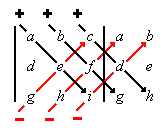
\includegraphics[scale=0.6]{sarrus}\\

\textbf{arithmetic rules:}\\
$\det (A \cdot B) = \det (A) \cdot \det (B)$\\
$\det (A^{-1}) = \det (A)^{-1}$\\
$\det\left(rA\right) = r^n\det A\,\,$,  for all $A^{n\times n}$ and scalars $r$

\subsection{rank}
Let A be a matrix.\\
$\text{rank}(A) = \text{columnSpace}(A) = \text{rowSpace}(A)$ \\
\quad = number of linearly independent column vectors of A\\
\quad = number of non-zero rows in A after applying Gauss\\

\subsection{row space}
The row space of a matrix is the set of all possible linear combinations of its row vectors.\\
Let $A$ be a matrix and $R$ a row-echelon form of $A$.\\
Then the set of nonzero rows in $R$ is a basis for the row space of $A$.

\subsection{column space}
Let $A$ be a matrix and $R$ a row-echelon form of $A$.\\
A basis for the column space of $A$ can be obtained by taking the columns of $A$ that correspond to the columns with leading entries in $R$.

\subsection{kernel == nullspace}
$\text{kern}(A) = \left\{ x\in\mathbb{R}^n : Ax = 0 \right\}$ \quad (the set of vectors mapping to 0)\\

\sect{rank and nullity}
$rank(A) + nullity(A) = n$\\

\subsection{trace}
defined on n$\times$n square matrices: $\mathrm{tr}(A) = a_{11} + a_{22} + \dots + a_{nn}$\\
(sum of the elements on the main diagonal)


\subsection{span}
Let $v_1,\dots,v_r$ be the column vectors of A. Then:\\
The span of $A$ may be defined as the set of all finite linear combinations of elements of $A$.\\
$\operatorname{span}(A) =  \{ {\lambda _1 v_1  +  \dots  + \lambda _r v_r \mid \lambda _1 , \dots ,\lambda _r  \in \mathbb{R}} \}$

\subsection{properties}
\textbf{square}: $N \times N$\\
\textbf{symmetric}: $A = A^T$\\
\textbf{diagonal}: 0 except $a_{kk}$\\

\sect{orthogonal} $A^T = A^{-1}$
$\Rightarrow$ normal and diagonalizable\\

\sect{nonsingular}
$A^{n \times n}$ is nonsingular = invertible iff:\\
\begin{itemize}
\item There is a matrix $B := A^{-1}$ such that $AB = I = BA$\\
\item $det(A) \ne 0$\\
\item $Ax = b$ has exactly one solution for each $b$, $b = 0$ included\\
\item The reduced row-echelon form of $A$ is an identity matrix\\
\item $A$ can be expressed as a product of elementary matrices.\\
\item The column vectors of $A$ are linearly independent\\
\item The rows of $A$ form a basis for $\mathbb{R}^{n}$\\
\item The columns of $A$ form a basis for $\mathbb{R}^{n}$\\
\item $\text{rank}(A) = n$\\
\end{itemize}

\smallbreak
$\Rightarrow det(A^{-1}) = \frac{1}{det(A)}$\\
$\Rightarrow (A^{-1})^{-1} = A$\\
$\Rightarrow (A^{T})^{-1} = (A^{-1})^{T}$

\sect{block matrices}
Let B, C be submatrices, and A, D square submatrices. Then:\\
$\det\begin{pmatrix}A& 0\\ C& D\end{pmatrix} = \det\begin{pmatrix}A& B\\ 0& D\end{pmatrix} = \det(A) \det(D)$

\sect{permutation matrix}
Permutation matrix $P = R_{k} \dots R_{1}$.\\
Row swap matrices $R_{i}$ are symmetric and that they are their own inverses.\\
$P^{-1} = R_{1} \dots R_{k} = R_{1}^{T} \dots R_{k}^{T}$.\\
Thus $P^{-1} = P^{T}$.

\sect{transpose properties}
$(A^T)^T = A$\\
$(AB)^T = A^TB^T$\\
$det(A^T) = det(A)$\\
$(A^T)^{-1} = (A^{-1})^T$

\subsection{compute powers}
$A = BDB^{-1}$. $D$ is a diagonal matrix.\\
$A^{n} = BD^{n}B^{-1}$.\\
$\begin{bmatrix}0& 1\\ 1& 1\end{bmatrix} = B \begin{bmatrix}\phi_{+}& 0\\ 0& \phi_{-1}\end{bmatrix}B^{-1}$\\
$\phi_{+} = \frac{1 + \sqrt{5}}{2}$; $\phi_{-} = \frac{1 - \sqrt{5}}{2}$; $\phi_{+}\phi_{-} = -1$\\
$B = \begin{bmatrix}1& 1\\ \phi_{+}& \phi_{-}\end{bmatrix}$\\
$B^{-1} = \frac{1}{\phi_{+} - \phi_{-}} \begin{bmatrix}-\phi_{-}& 1\\ \phi_{+}& -1\end{bmatrix}$\\
$fib[n] = \frac{\phi_{+}^{n} - \phi_{-}^{n}}{\phi_{+} - \phi_{-}}$
$\begin{bmatrix}0& 1\\ 1& 1\end{bmatrix}^{n} = \frac{1}{\phi_{-} - \phi_{+}}\begin{bmatrix}\phi_{+}^{n-1} - \phi_{-}^{n-1}& \phi_{-}^{n} - \phi_{+}^{n}\\ \phi_{-}^{n} - \phi_{+}^{n}& -\phi_{+}^{n+1} + \phi_{-}^{n+1}\end{bmatrix}$

\subsection{Cramer’s Rule}
$Ax = b$\\
$x_{1} = \frac{det(A_{1 \leftarrow b})}{det(A)}$
$x_{2} = \frac{det(A_{2 \leftarrow b})}{det(A)}$
$x_{3} = \frac{det(A_{3 \leftarrow b})}{det(A)}$

\subsection{Cofactor}
Let $M_{ij}$ be the matrix $A$ with the $i^{th}$ row and $j^{th}$ column removed.\\
$C_{ij} = (-1)^{i+j}det(M_{ij})$\\
$det(A) = \sum_{j=1}^{n}(-1)^{i+j}a_{ij}det(M_{ij})$\\
$A^{-1} = \frac{C^{T}}{det(A)} \Rightarrow AC^{T} = det(A)I_{n}$

\subsection{Orthogonality}
Two vectors are orthogonal if and only if\\
$u^{T}v = 0$

\subsection{subset vs subspace}
A subset is just a set of elements from the vector space.\\
A subspace of a vector space is a subset that follow the 3 rules.

\sect{subspace}
The $\cap$ of two subspaces of $\mathbb{R}^{n}$ is still a subspace of $\mathbb{R}^{n}$.\\
The $\cup$ of two subspaces of $\mathbb{R}^{n}$ may not be a subspace of $\mathbb{R}^{n}$.

\subsection{dimension}
The dimension of a vector space $V$ , denoted by $dim(V)$, is defined to be the number of vectors in a basis for $V$.\\
In addition, we define the dimension of the zero space to be zero.

\sect{solving $[A|b]$}
Do Gaussian elimination on the augmented matrix $[A|b]$.\\
If $rank([A|b]) > rank(A) \Rightarrow Ax = b \text{ does not have a solution} \Rightarrow \text{b is not in the column space of } A$

\subsection{dimension general case}
Vector space $M(m, n)$ of all m-by-n matrices.\\
The dimension of this space is $m \times n$\\
Let $E_{ij}$ be the m-by-n matrix that is all zero except for a 1 in the $(i, j)$ entry.\\
The all the $E$ matrices are a basis for $M(m, n)$

\subsection{Reasoning about dimension}
Let $S \subseteq \mathbb{R}^{n}$ be a subspace:\\
\quad if vectors $v_{1}, \dots, v_{k} \in S$ are linearly independent, then\\
\quad \quad $dim(S) \geq k$\\
\quad if $span({v_{1}, \dots, v_{k}}) = S$ then\\
\quad \quad $dim(S) \leq k$

\subsection{General solution for $Ax = b$}
$x$ = (the general solution of $Ax = 0$)\\
\quad $+$ (one particular solution of $Ax = b$).\\
e.g\\
$x = s*v_{1} + t*v_{2} + a$\\ $v_{i}$ spans nullspace of $A$\\$a$ is a particular solution.
\end{multicols}
\end{document}